\documentclass[12pt, a4paper]{article}
\usepackage[utf8]{inputenc}
\usepackage[T1]{fontenc}
\usepackage[swedish]{babel}
\usepackage{fullpage}
\usepackage{amsmath}
\usepackage{amsfonts}
\usepackage{tkz-euclide}
\usepackage{changepage,lipsum,titlesec}% http://ctan.org/pkg/{changepage,lipsum,titlesec}
\usepackage{graphicx}
\usepackage{color}

\titleformat{\section}[block]{\LARGE\bfseries}{\thesection.}{1em}{}
\titleformat{\subsection}[block]{\Large\bfseries}{\thesubsection}{1em}{}
\titleformat{\subsubsection}[block]{\large\bfseries}{\thesubsubsection}{1em}{}
\titlespacing*{\subsection} {2em}{3.25ex plus 1ex minus .2ex}{1.5ex plus .2ex}
\titlespacing*{\subsubsection} {3em}{3.25ex plus 1ex minus .2ex}{1.5ex plus .2ex}

\makeatletter
  %\edef\g@prae{\hfil$}
  %\edef\g@post{$}
\makeatother

\newcommand{\BAR}{%
  \hspace{-\arraycolsep}%
  \strut\vrule % the `\vrule` is as high and deep as a strut
  \hspace{-\arraycolsep}%
}

\makeatletter
\def\myline{\pgfutil@ifnextchar[{\my@line}{\my@line[]}}%
\def\my@line[#1](#2)(#3){%
\tikz[remember picture,overlay] \draw[#1]  (#2)--(#3); 
}%
\newcommand\mypoint[1] {%
\tikz[remember picture] \path coordinate (#1);}% 

\begin{document}


	\title{
		\textbf{Sudoku}
	}

	\author{Adil Arzhane 930905-4337, Erik Englund 921016-4530, Oskar Persson 940120-8237\\Program Design and Data Structures 2013/2014}
	\maketitle

	
\begin{tikzpicture}[remember picture, overlay]
      \node[draw,minimum width=4in,rotate=-45,fill=orange,text=white,font=\large] at ($(current page.north east) + (-1.1in,-1.1in)$) {Adil är sämst};
      \node[draw,minimum width=4in,rotate=45,fill=orange,text=white,font=\LARGE] at ($(current page.north west) + (0.9in,-0.9in) $) {Adil är sämst};
      \node[draw,minimum width=4in,rotate=-45,fill=orange,text=white,font=\LARGE] at ($(current page.south west) + (0.9in,0.9in) $) {Adil är sämst};
      \node[draw,minimum width=4in,rotate=45,fill=orange,text=white,font=\LARGE] at ($(current page.south east) + (-0.9in,0.9in) $) {Adil är sämst};
    \end{tikzpicture}

	\tableofcontents
	\newpage

	\section{Introduction}
	\begin{adjustwidth}{2em}{0pt}
		\subsection{What is a Sudoku?}
			\begin{adjustwidth}{3em}{0pt}
				A sudoku is a numeric puzzle made out of a nine-by-nine grid where each row, column and three-by-three-subsection contains unique numbers from 1 to 9. The idea is that you start with a puzzle where some numbers are missing and the goal is to find out which numbers they are. An example of a typical non-solved sudoku is shown below. \\
				\begin{center}
					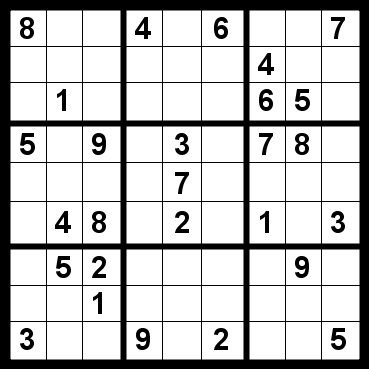
\includegraphics[width=3in]{puzzle.png} \\ \textit{Figure 1}
				\end{center}

				In this project, we have focused on creating a data-program intended to solve a given sudoku-puzzle.
	  		\end{adjustwidth}
	\end{adjustwidth}
  	\newpage
  	\section{User Guidelines}
		\begin{adjustwidth}{3em}{0pt}
			\textbf{Requirements:} PolyML \\
			\textbf{Instructions:} 
			In order to solve the sudoku shown in figure 1, using our application, you must give the program the following input, in the terminal: \\
			\begin{ttfamily}
				> cd /path/to/folder/containing/application \\
				> poly \\
				> use “sudoku.sml”; \\
				> val h = {[}{[}8,0,0,4,0,6,0,0,7{]},
					\begin{adjustwidth}{5.5em}{0pt}
				           {[}0,0,0,0,0,0,4,0,0{]}, \\
					       {[}0,1,0,0,0,0,6,5,0{]}, \\
				           {[}5,0,9,0,3,0,7,8,0{]}, \\
				           {[}0,0,0,0,7,0,0,0,0{]}, \\
					       {[}0,4,8,0,2,0,1,0,3{]}, \\
				           {[}0,5,2,0,0,0,0,9,0{]}, \\
				           {[}0,0,1,0,0,0,0,0,0{]}, \\
				           {[}3,0,0,9,0,2,0,0,5{]}{]}; \\
				    \end{adjustwidth}
				> val s = createPuzzleFromHorizontal h; \\
				> solve s;\\
			\end{ttfamily}

			\textbf{Running test-cases:} In order to run the test-cases you must give the following input, in the terminal:\\
			\begin{ttfamily}
				> cd /path/to/folder/containing/application \\
				> poly \\
				> use “sudoku.sml”; \\
				> use “sudoku\_tests.sml”; \\
				> tests (); \\
			\end{ttfamily}
  		\end{adjustwidth}

  	\section{Implmentation}
	\begin{adjustwidth}{2em}{0pt}
		\subsection{Algorithms}
			\begin{adjustwidth}{3em}{0pt}
				When we started out the project, the first thing we did was figuring out how we would solve a sudoku by hand, which operations we would carry out and in which order. We figured that the first thing we would do was to look whether the same number occurred two times in the same three by three horizontal row or vertical column. This would mean that the third occurrence of this number should be inserted into the column or row that the previous two did not already cover.

				In the puzzle shown above (fig. 1) we would for example find that number 5 is occurring in the first and second vertical columns (counting from left to right). Since they are located in the fourth and seventh three-by-three square (counting from top left to bottom right), the 5 in the third vertical column should be located in the first three-by-three square.

				The next step would be to check the horizontal rows related to the first three-by-three   square (from here on in called square) to see whether there are any 5’s that cuts away any of the three possible positions in the first square. We see that there is only one 5 located in the three top-most horizontal rows and therefore we have two possible spots for the 5 in the first square. From here we cannot proceed any further, and we have to look at other columns and numbers too see if we can find a position where we only have one option. 

				In the example we can see that there is a 1 occurring in the second and third vertical columns, and a 1 in the sixth horizontal row (counting top to bottom). This means there is only one option for the 1 in the first vertical column, and we can fill that in and continue with other numbers and positions.

				However, if you start out with a puzzle where you can make no conclusions by using the algorithm above, you have to approach the puzzle from a slightly different angle. By looking at which square that contains the most amount of known numbers, you can produce all possible permutations of that single square and see which one of them that works together with the rest of the puzzle (ie. no number occurs more than once in the same square, row or column). By doing this, you might have to try and solve the puzzle with one permutation at a time to see which one of them “works out”. This might be relatively time consuming given that in worst case your last permutation is the right one. On the other hand, if you’re lucky you will get it right at the first try.

				This is the operations we decided to try and implement into our program code for solving sudokus. However, we ended up using an algorithm where we first search for a single unknown element, and if there are none we use the traversing function to find a possible solution.


	  		\end{adjustwidth}
	  	\subsection{Tree Structure}
			\begin{adjustwidth}{3em}{0pt}
				In our code, we chose to represent possible solutions to a sudoku puzzle in a tree structure, a \begin{ttfamily}STree\end{ttfamily}, consisting of a root that is the puzzle handled at the moment and a list of \begin{ttfamily}STrees\end{ttfamily} that holds all potential next steps to the puzzle.

				\begin{center}
					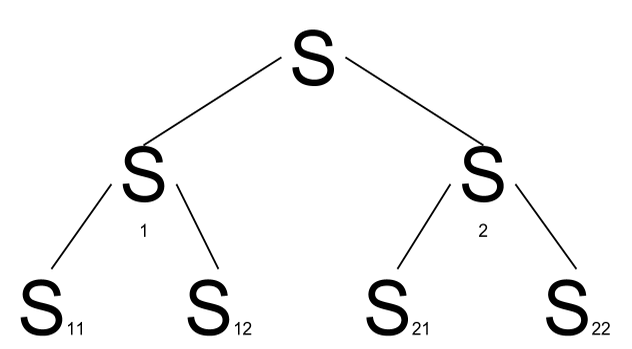
\includegraphics[width=3in]{tree.png} \\ \textit{Figure 2}
				\end{center}

				In \textit{figure 2} we see that $S$ is the puzzle from the start. $S_1$ and $S_2$ are both next potential steps to $S$. $S_{11}$ and $S_{12}$ are potential steps to $S_1$ and so on. So what the algorithm will do is start at $S$ and check if it can easily fill in single missing numbers on rows, columns or squares. Then it get all the permutations of the square with the least amount of unknowns and creates the potential next steps $S_1$ and $S_2$. Then it first goes into $S_1$ and checks if it has any potential next steps. If it doesn’t then it goes to check into $S_2$. It will continue doing this until it finds a solution or if it has checked every potential one.

			\end{adjustwidth}

		\subsection{Datatypes}
			\begin{adjustwidth}{3em}{0pt}
				For this project, we have chosen to represent a sudoku as a datatype in SML consisting of three lists of integer lists. One of the lists represents the horizontal rows, another the vertical columns and the third the 9 different three-by-three squares.

			\end{adjustwidth}

		\subsection{Functions}
			\begin{adjustwidth}{3em}{0pt}
				\subsubsection{ascii}
					\begin{adjustwidth}{3em}{0pt}
						The function \begin{ttfamily}ascii\end{ttfamily} is used to easier get a better overview of the sudoku. The function takes a puzzle and prints this in the structure of a sudoku, a nine-by-nine grid with three-by-three squares as subsections.
					\end{adjustwidth}

				\subsubsection{sumOfElements}
					\begin{adjustwidth}{3em}{0pt}
						\begin{ttfamily}sumOfElements\end{ttfamily} is used to receive the total sum of a list of integers, this function is mostly used to find the total value of a three-by-three square. Since the sum of all integers 1-9 is 45, we know that each square must have a total value of 45 in order to be stated as solved.
					\end{adjustwidth}

				\subsubsection{oneUnknown}
					\begin{adjustwidth}{3em}{0pt}
						If there is a single zero (0) in a list, \begin{ttfamily}oneUnknown\end{ttfamily} will replace this element with the missing integer (1-9).
					\end{adjustwidth}
				\subsubsection{notInSquare}
					\begin{adjustwidth}{3em}{0pt}
						Lists the numbers from 1-9 that is missing from a list, so that we know what numbers we have, and which are missing and need to be filled in.
					\end{adjustwidth}
				\subsubsection{permute}
					\begin{adjustwidth}{3em}{0pt}
						Returns all permutations of the integer list used, a permutation is a combination of a list of numbers. This code was taken from \\ http://stackoverflow.com/questions/4102605/ \\standard-ml-permutations/5631165
					\end{adjustwidth}
				\subsubsection{squareWithLeastUnknowns}
					\begin{adjustwidth}{3em}{0pt}
						This function is used to find the first square in the sudoku with the least unknowns in it.

					\end{adjustwidth}
				\subsubsection{possibleSolutionsForSquare}
					\begin{adjustwidth}{3em}{0pt}
						Is used to receive possible solutions for squares (pretty much as the name says) by using the permutations. 
					\end{adjustwidth}
				\subsubsection{traversal}
					\begin{adjustwidth}{3em}{0pt}
						\begin{ttfamily}traversal\end{ttfamily} is the main function of the program. By using the previous mentioned functions, it will traverse through a \begin{ttfamily}STree\end{ttfamily}  containing all possible permutations in each step towards the solution.
					\end{adjustwidth}
			\end{adjustwidth}
		\subsection{Test cases}
			\begin{adjustwidth}{3em}{0pt}
				See enclosed test code (\begin{ttfamily}sudoku\_tests.sml\end{ttfamily}).
			\end{adjustwidth}
	\end{adjustwidth}

	\section{Discussion}
		\begin{adjustwidth}{3em}{0pt}
			When we started this project our goal was to create a program that would be able to solve any sudoku in reasonable time, whether the sudoku was considered easy or extremely hard. Naturally we chose to start at the bottom with simple lists to get a working algorithm that would not take too long. When we had written the code and it worked, we encountered a slight problem. The algorithm took too long time to solve these sudokus. A sudoku considered easy, medium or hard took about 30-40 seconds to solve, and a sudoku considered one of the world’s hardest took us 6 hours.

			We continued to work with vectors in our code instead of lists, figuring we might be able to  solve sudokus faster, since elements in a vector can be accessed in constant time regardless of where in the vector it is located. The downside is that if you need to replace an element in a vector you have to rebuild the whole vector.

			When we had completed the work with vectors, we saw that the result was not what we had set out for. The time needed to solve the same puzzles as we solved with lists was almost three times longer. A possible cause of this problem might be that we build new vectors more often than we access elements (ie the code writes to more vectors than it reads), which causes the code to run slower with vectors than with lists.

			After a meeting with our supervisor we realized that our algorithm and implementation would not work faster just with vectors, but that we had to use ref vectors, since ref vectors allows you to both read and update in constant time. This would, in theory, increase the algorithms efficiency and the code would run much faster and smoother.

			The implementation of ref vectors were succeeded and we ran our test cases to see if our hypothesis were correct. Even if we would have loved the program to run faster it did not. ref vectors took even longer than normal vectors, we had a problem. After implementing three different versions: int list list, int vector vector, int ref vector vector and finally int ref vector ref vector we saw that the first was also the fastest. The reason that the list implementation was the fastest was that we implemented the functions with lists in mind. If we had gone with another data structure from the start and built the functions around that, then those would have been faster.
		\end{adjustwidth}

	\section{Possible Improvements}
		\begin{adjustwidth}{3em}{0pt}
			The main problem with solving sudokus is the time taken to solve harder puzzles. With our algorithm, using lists, it takes approximately 6 hours to solve the hardest puzzle we could find, while a “standard” puzzle requires between 20-40 seconds depending on difficulty. When using vectors, it took even longer to solve the same puzzles. The most probable reason to this is that we started out writing our code using lists, and then we reworked the same code using vectors. If we had started over from the beginning, implementing the algorithm with vectors we might have reached a different result.

			Another thing to try is before all permutations is created in the function permute, try to not even create the permutations that will not work. Currently all possible permutations is created and then those that won’t work are removed.
		\end{adjustwidth}
		
	\section{Summary}
		\begin{adjustwidth}{3em}{0pt}
			To sum it all up, we have an algorithm that goes through each possible solution to the given sudoku and stops when it finds one that works. We went with lists since that is the fastest one and the implementation was built around it.
		\end{adjustwidth}
	
	\section{References}
		\begin{adjustwidth}{3em}{0pt}
			\begin{itemize}
				\item{http://stackoverflow.com/questions/4102605/standard-ml-permutations\\/5631165}
				\item{http://standardml.org/Basis/list.html}
				\item{http://standardml.org/Basis/vector.html}
				\item{http://standardml.org/Basis/time.html}
			\end{itemize}
		\end{adjustwidth}

	\section{Diaries}
		\begin{adjustwidth}{3em}{0pt}
			Time spent (from github commits https://github.com/Oskwish/Sudoku/commits/master)
			
				\begin{table}[h]
					\begin{adjustwidth}{3em}{0pt}
						\begin{center}
							\begin{tabular}{|c|c|c|}
								\hline
								Oskar Persson & 59 hours & 30 minutes \\ \hline
								Erik Englund  & 52 hours & 30 minutes \\ \hline
								Adil Arhzane  & 38 hours & 15 minutes \\ \hline
							\end{tabular}
						\end{center}
					\end{adjustwidth}
				\end{table}
			
		\end{adjustwidth}


\end{document}